\documentclass[a4paper]{article}
\usepackage[utf8]{inputenc}
\usepackage{braket}
\usepackage{amsmath}
\usepackage{graphicx}
\usepackage{float}
\usepackage{soul}
\usepackage{caption}
\usepackage[subrefformat=parens,labelformat=parens]{subcaption}
\usepackage{wrapfig}
\usepackage{geometry}
\usepackage{derivative}

\usepackage{hyperref}
\hypersetup{
colorlinks=true,
linkcolor=blue,
citecolor=blue,
filecolor=green,
urlcolor=blue,
}

\newgeometry{margin=3cm}

\graphicspath{ {../plots} }

\newcommand{\threejm}[6]{ \left(\begin{array}{ccc} #1 & #3 & #5\\
    #2 & #4 & #6
\end{array}
\right)}
\newcommand{\sixj}[6]{ \left\{\begin{array}{ccc} #1 & #3 & #5\\
    #2 & #4 & #6
\end{array}
\right\}}
\newcommand{\ninej}[9]{\left\{\begin{array}{ccc}
#1 & #2 & #3\\
#4 & #5 & #6\\
#7 & #8 & #9
\end{array}
\right\}}


\title{Calculation of diatom-atom collisions in a magnetic field}
\author{Marcin Welter}

\begin{document}
\maketitle


\section{Alkali like atom + atom collision}\label{sec:atom_atom}
    For the problem of collision of two alkali like atoms A + B we consider following Hamiltonian
    \begin{equation}
        \hat{H} = -\frac{1}{2\mu}\pdv[order=2]{}{R} + \frac{\hat{L}^2}{2\mu R^2}
            + \hat{H}^\text{A}_\text{int} + \hat{H}^\text{B}_\text{int} + \hat{V}(R),
    \end{equation}
    where $R$ is the distance between atoms, $\mu$ is the reduced mass of two atoms, 
    \(\hat{L}^2\) is the angular momentum of the two atoms,
    \(\hat{H}^k_\text{int}\) is the internal structure of a k atom and \(\hat{V}(R)\) 
    consists of triplet and singlet potential curves.

\subsection{Hyperfine and Zeeman structure}
    Internal structure of alkali like atoms in the magnetic field consists of Zeeman splitting and
    hyperfine structure. The internal hamiltonian for such atom $k$ is written as
    \begin{equation}\label{eq:alkali_hamiltonian_int}
        \hat{H}^k_\text{int} = \hat{H}^k_\text{Zee} + \hat{H}^k_\text{hf},
    \end{equation}
    with \(\hat{H}^k_\text{Zee} = -\gamma_e B \hat{s}^k_z - \gamma^k_n B \hat{i}^k_z\) and 
    \(\hat{H}^k_\text{hf} = a^k_\text{hf} \ \hat{\mathbf{s}}^k \cdot \hat{\mathbf{i}}^k\).

    In the basis \(\ket{s m_s i m_i} \equiv \ket{m_s m_i}\) the matrix elements of the internal Hamiltonian are
    \begin{equation}
        \braket{m_s m_i | H^k_\text{Zee} | m'_s m'_i} = -B(\gamma_e m_s + \gamma^k_n m_i) \delta^{m'_s m'_i}_{m_s m_i},
    \end{equation}
    for Zeeman part and the hyperfine part is
    \begin{equation}
        \braket{m_s m_i | H^k_\text{hf} | m'_s m'_i} = a^k_\text{hf} 
            \left(
                m_s m_i \delta_{m_s m_i}^{m'_s m'_i} 
                + \frac{1}{2}\sum_{p = \pm 1} C(s, m_s, m'_s) C(i, m_i, m'_i)\delta_{m_s m_i}^{m'_s + p, m'_i - p}
            \right),
    \end{equation}
    where \(C(s, m_s, m'_s) = \sqrt{s(s + 1) - m_s m'_s}\). 
    We see that the total projection $m_f = m_i + m_s$ is preserved.

\subsection{Singlet and triplet potential curves}
    Potential term consists of singlet and triplet potential curves, we can write it as
    \begin{equation}
        \hat{V}(R) = \hat{\mathcal{P}}_1 V_1(R) + \hat{\mathcal{P}_0} V_0(R),
    \end{equation}
    where \(\mathcal{P}_S\) is a projection to the subspace with combined electron spin of two atoms equal to $S$
    and \(V_S(R)\) is a corresponding potential curve.

    In the electron spin basis \(\ket{m_s^\text{A}, m_s^\text{B}}\) of each atom,
    the matrix elements of the projection operator are
    \begin{equation}
        \braket{m_s^\text{A} m_s^\text{B} | \mathcal{P}_S | m_s^{'\text{A}} m_s^{'\text{B}}}
            = \sum_{M_S} \braket{m_s^\text{A} m_s^\text{B} | S M_S}\!\braket{S M_S| m_s^{'\text{A}} m_s^{'\text{B}}}.
    \end{equation}

\subsection{Full basis}
    Full basis is then \(\ket{m_s^\text{A} m_s^\text{B} m_i^\text{A} m_i^\text{B}}\) with total spin projection \(M_F\) being conserved.
    Additionally, angular momentum and its projection are good quantum numbers.
    For homo-nuclear we can transform the basis to the combined electron and nuclear spin for which the symmetry is evident
    and we restrict ourselves to only the needed symmetry of the system.

\section{Spinless rigid rotor + atom collision}
    Here we consider a diatom + atom collision without spin structure in a rigid rotor approximation.
    The Hamiltonian for such a system is
    \begin{equation}
        \hat{H} = -\frac{1}{2\mu}\pdv[order=2]{}{R} + \frac{\hat{L}^2}{2\mu R^2} + \hat{H}_\text{rot} + V(R, \theta)
    \end{equation}
    where $R, \theta$ are the Jacobi coordinates, $\mu$ is the reduced mass of the atom and diatom, 
    \(\hat{L}^2\) is the orbital angular momentum of the system,
    \(\hat{H}_\text{rot}\) is the Hamiltonian of the rigid-rotor and \(\hat{V}(R, \theta)\) 
    is the potential surface.

    Rigid rotor Hamiltonian is
    \begin{equation}
        \hat{H}_\text{rot} = B_e \hat{N}^2,
    \end{equation}
    where \(B_e\) is a rotational constant of the rotor.

    We work in \(\ket{(lN)J M_J}\) basis being the combined angular momentum basis \(J\) of orbital angular momentum of the system
    \(l\) and rotation of the molecule \(N\).
    In this basis the matrix elements of the potential terms are
    \begin{equation}
        \braket{(lN)J M_J |V(R, \theta)| (l'N')J' M'_J} = \sum_\lambda V_\lambda(R) f_\lambda(lN, l'N'; J) \delta^{JM_J}_{J'M'_J},
    \end{equation}
    where $V_\lambda(R)$ is the $\lambda$-th term of the Legendre decomposition of the potential $V(R, \theta)$
    and
    \begin{multline}
        f_\lambda(lN, l'N'; J) = (-1)^{l + l' + J} \sqrt{(2N + 1)(2N' + 1)(2l + 1)(2l' + 1)} \\
            \times \threejm{l}{0}{\lambda}{0}{l'}{0} \threejm{N}{0}{\lambda}{0}{N'}{0} \sixj{l}{N'}{\lambda}{J}{l'}{N},
    \end{multline}
    are the Percival-Seaton coefficients.
    Other terms in the Hamiltonian are straightforward and total angular momentum \(J\) 
    and its projection is conserved \(M_J\).
    Additionally if the potential only have even numbered terms in the Legendre decomposition,
    divisibility of \(l, N\) by two is conserved.

\section{Alkali like rigid rotor + atom collision}
    We now consider a alkali like diatom + atom collision, by that we mean
    that the diatom consists of alkali like atom and a structureless atom that collide with the alkali like atom.
    The Hamiltonian for such a system, following Ref. \cite{tscherbul2023ultracold} is
    \begin{equation}
        \hat{H} = -\frac{1}{2\mu}\pdv[order=2]{}{R} + \frac{\hat{L}^2}{2\mu R^2} 
            + \hat{H}^\text{rot}_\text{int} + \hat{H}^\text{A}_\text{int} 
            + \hat{\mathcal{P}}_1 V_1(R, \theta) + \hat{\mathcal{P}_0} V_0(R, \theta),
    \end{equation}
    where internal atom Hamiltonian and projection operators are the same as in Sec. \ref{sec:atom_atom}
    and the internal rotor hamiltonian can be further written as
    \begin{equation}
        \hat{H}^\text{rot}_\text{int} = \hat{H}_\text{rot} + \hat{H}_\text{spin-rot} 
            + \hat{H}_\text{ahf} + \hat{H}_\text{spin}.
    \end{equation}

    The first term is the same as without the spin that is \(\hat{H}_\text{rot} = B_e \hat{N}^2\),
    second term is the coupling between rotor rotation and electron spin of the rotor
    \begin{equation}
        \hat{H}_\text{spin-rot} =  \gamma_\text{sr} \hat{\mathbf{N}}\cdot \hat{\mathbf{s}}^\text{r},
    \end{equation}
    where \(\gamma_\text{sr}\) is a spin-rot coupling constant,
    \begin{equation}
        \hat{H}_\text{ahf} = \frac{c\sqrt{6}}{3} \left(\frac{4 \pi}{5}\right) ^ {1 / 2}
        \sum_{q=-2}^2 (-1)^qY_{2-q}(\theta_r,\phi_r) [\hat{\mathbf{i}}^\text{r} \otimes \hat{\mathbf{s}}^\text{r}]^{(2)}_q,
    \end{equation}
    is an anisotropic hyperfine contribution with anisotropic hyperfine constant being \(c\).
    Last term is the hyperfine and Zeeman structure same as discussed for the atom case.

    The basis used is \(\ket{(l N) J M_J} \! \ket{(s^r) m_s^r} \ket{(i^r) m_i^r} \ket{(s^a) m_s^a} \ket{(i^a) m_i^a}\).
    In this basis, matrix elements of the spin-rot contribution are
    \begin{multline}\label{eq:spin_rot_mel}
        \braket{(lN) J M_J |\langle m_s^r | \hat{H}_\text{spin-rot} | (l'N') J M_J \rangle| m_s'^r}
            = \delta_{lN}^{l'N'} \gamma_\text{sr} p_3(N)p_3(s^r) [(2J+1)(2J'+1)]^{1/2}
            \\ \times \sum_p (-1)^{p} (-1)^{J-M_J}(-1)^{N+l+J'+1} (-1)^{s^r - m_s^r}
            \\ \times \sixj{N}{J'}{J}{N}{l}{1} \threejm{J}{-M_J}{1}{p}{J'}{M_J'} \threejm{s^r}{-m_s^r}{1}{-p}{s^r}{m_s'^r} 
    \end{multline}
    where \(p_3(X) = \sqrt{X(2X + 1)(X + 1)}\) and 
    matrix elements of the anisotropic hyperfine contribution are
    \begin{multline}\label{eq:anisotropic_hifi_mel}
        \braket{(lN)J M_J |\langle m_s^r m_i^r | \hat{H}_\text{ahf} | (l'N') J'M'_J\rangle| m_s'^r m_i'^r} \\
            = \delta_{ll'} c\frac{\sqrt{30}}{3} (-1)^{J - M_J + l + J'}
            p_3(i^r) p_3(s^r) [(2J + 1)(2J' + 1)] ^ {1/2} [(2N + 1)(2N' + 1)] ^ {1/2} 
            \\ \times\sixj{N}{J'}{J}{N'}{l}{2}  
                \threejm{1}{m_i^r - m_i'^r}{1}{m_s^r - m_s'^r}{2}{M_J - M_J'} 
                \threejm{N}{0}{2}{0}{N'}{0} 
            \\ \times \threejm{J}{-M_J}{2}{M_J - M_J'}{J'}{M_J'}
            \threejm{i^r}{-m_i^r}{1}{m_i^r - m_i'^r}{i^r}{m_i'^r}
            \threejm{s^r}{-m_s^r}{1}{m_s - m_s'^r}{s^r}{m_s'^r}.
    \end{multline}

\section{Reconstructing results}
\subsection{Two Li\(^6\) feshbach resonances}
    \begin{figure}[H]
        \centering
        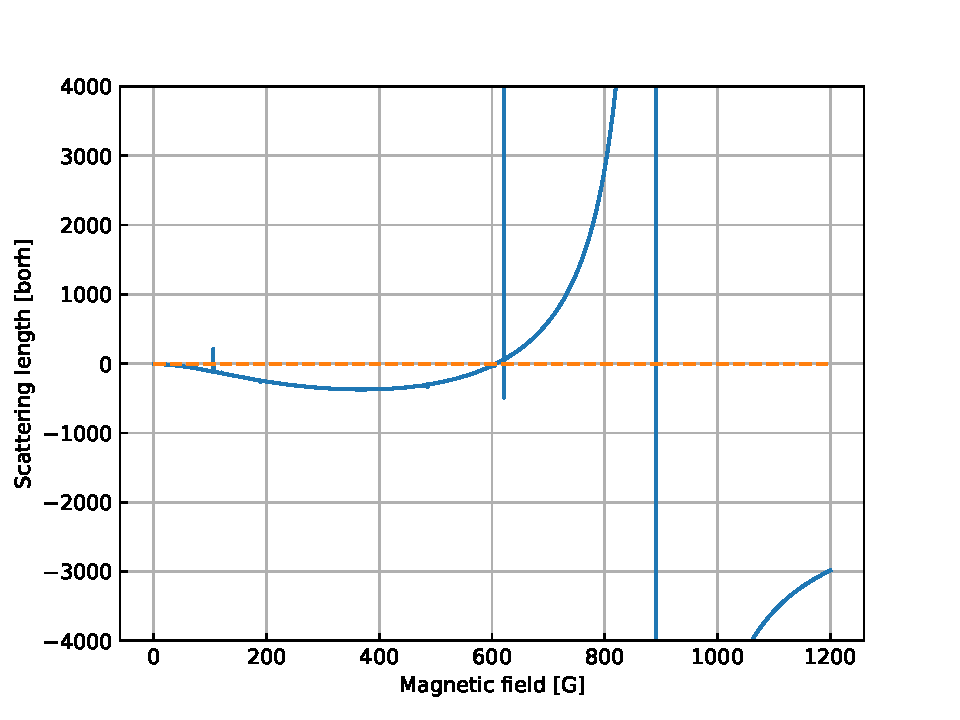
\includegraphics[width = 0.7\columnwidth]{li2_feshbach.pdf}
        \caption{Magnetic Feshbach resonances between two Li$_6$ in the lowest channel, 
            reconstruction of \cite{julienne2014contrasting}.
        }
        \label{fig:li6_feshbach}
    \end{figure}

\subsection{Spinless AlF + Rb cross sections}
    \begin{figure}[H]
        \centering
        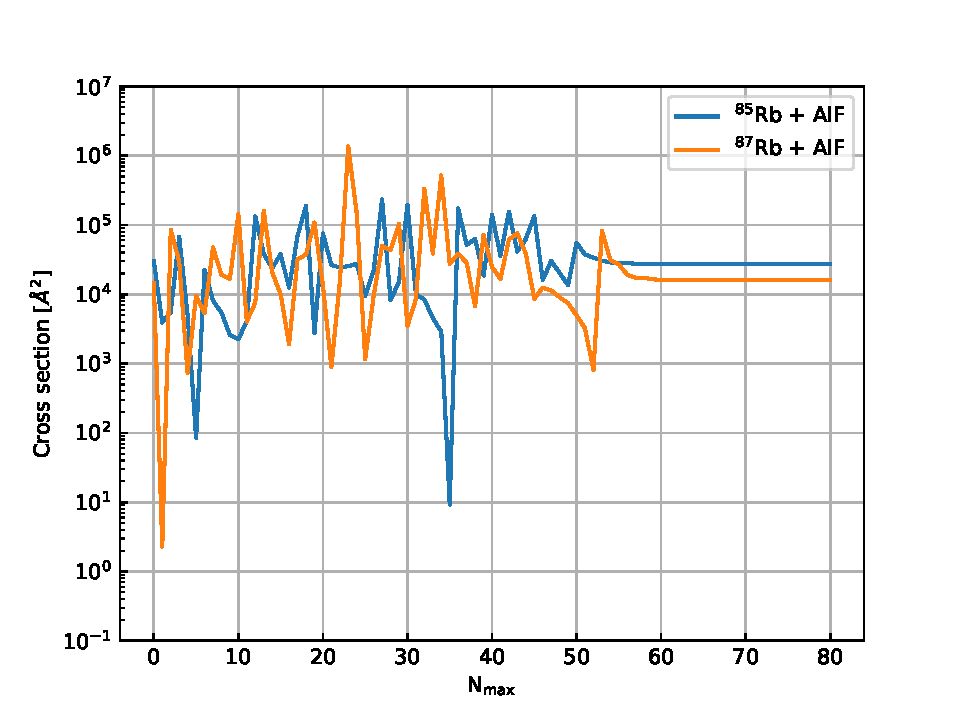
\includegraphics[width = 0.7\columnwidth]{spinless_AlF_Rb_n_max_dependence.pdf}
        \caption{Reconstruction of elastic cross section of AlF + Rb vs maximum value of \(N\).}
        \label{fig:alf_rb_sections}
    \end{figure}

\subsection{SrF + Rb Feshbach resonances}
    \begin{figure}[H]
        \centering
        \begin{subfigure}{.48\textwidth}
            \centering
            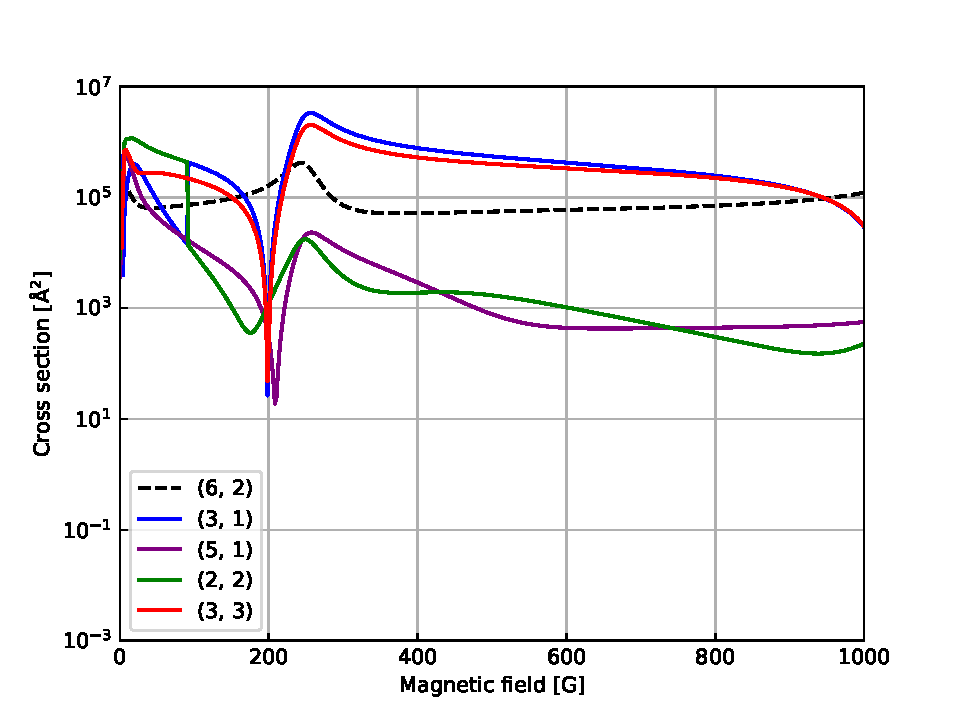
\includegraphics[width = 1\columnwidth]{SrF_Rb_scatterings_n_max_0.pdf}
            \caption{Calculation with $N_\text{max} = 0$}
        \end{subfigure}
        \begin{subfigure}{.48\textwidth}
            \centering
            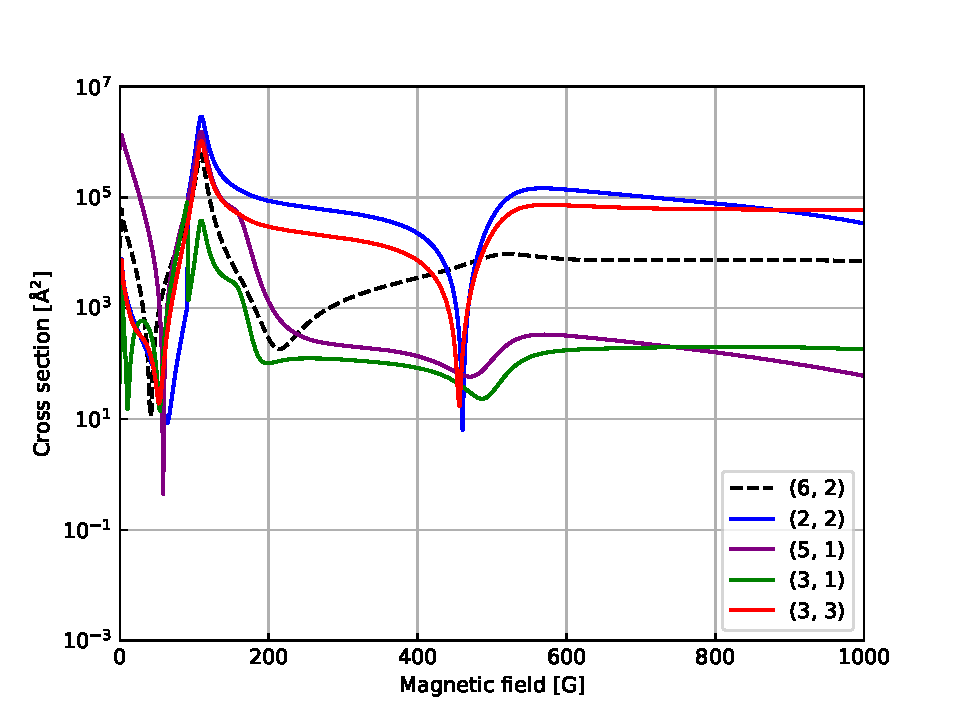
\includegraphics[width = 1\columnwidth]{SrF_Rb_scatterings_n_max_10.pdf}
            \caption{Calculation with $N_\text{max} = 10$}
    \end{subfigure}
    \label{fig:srf_rb_feshbach}
    \caption{Magnetic Feshbach resonances of SrF + Rb, 
        reconstruction of \cite{morita2024magnetic} in supplementary materials.
    }
    \end{figure}

    \bibliographystyle{unsrt}
    \bibliography{bibliography}
\end{document}